\documentclass[t]{beamer}
\usetheme{Copenhagen}
\setbeamertemplate{headline}{} % remove toc from headers
\beamertemplatenavigationsymbolsempty

\usepackage{amsmath, array, tikz, bm, pgfplots, tcolorbox, graphicx, venndiagram, color, colortbl}
\pgfplotsset{compat = 1.16}
\usepgfplotslibrary{statistics}
\usetikzlibrary{trees}

\title{Probability: OR}
\author{}
\date{}

\AtBeginSection[]
{
  \begin{frame}
    \frametitle{Objectives}
    \tableofcontents[currentsection]
  \end{frame}
}

\begin{document}

\begin{frame} 
\maketitle
\end{frame}

\section{Calculate probabilities using the Addition Rule}

\begin{frame}{AND vs. OR}
In the last section, we examined probabilities that focused on the word \textit{and}.	\newline\\	\pause

The word \textit{and} meant that we \alert{multiplied} the probabilities. \newline\\	\pause

In this section, we will focus on the word \textit{or}, which will mean \alert{adding} probabilities.
\end{frame}

\begin{frame}{Example 1}
A fair die is rolled. What is the probability of rolling a 4 or a 5.	\newline\\	\pause

Number of outcomes in the sample space: 6	\newline\\	\pause

What we want to happen: roll a 4 or a 5. This can happen in 2 ways. 

\begin{align*}
\onslide<4->{P(4\text{ or } 5) &= \frac{2}{6}} \\[8pt]
\onslide<5->{&= \frac{1}{3}}
\end{align*}
\end{frame}

\begin{frame}{The Addition Rule}
In the previous example, the events ``rolling a 4" and ``rolling a 5" were \emph{mutually exclusive}. \newline\\	

\onslide<2->{To find the \texttt{OR} probability of two mutually exclusive events, use the Addition Rule:}

\onslide<3->{\[P(A \text{ or } B) = P(A) + P(B)\]}
\end{frame}

\begin{frame}{Venn Diagram -- OR}
\begin{center}
\begin{venndiagram2sets}[shade=red!60]
\fillA \fillB
\node at (4.75,3.15) {$\mathcal{S}$};
\end{venndiagram2sets}
\end{center}
\[P(A \text{ or } B)\]
\end{frame}

\begin{frame}{Example 2}
The table below lists the types and numbers of cars sold at Lemon Autos along with their ages. Find each probability.	
\begin{center}
\begin{tabular}{c|ccccc}
					&	\textbf{0--2} & \textbf{3--5} & \textbf{6--10} & \textbf{Over 10} & \textbf{Total} \\ \hline
\textbf{Foreign} 	& 37 & 21 & 12 & 30 & 100 \\
\textbf{Domestic} 	& 35 & 23 & 11 & 31 & 100 \\ \hline
\textbf{Total}   	& 72 & 44 & 23 & 61 & 200
\end{tabular}
\end{center}
(a) \quad If a car is randomly selected, what is the probability that the car is 0--2 years old or over 10 years old?
\begin{align*}
\onslide<2->{P(\text{0--2 or over 10}) &= P(0-2) + P(\text{over 10})} \\
\onslide<3->{&= \frac{72}{200} + \frac{61}{200}} \\[8pt]
\onslide<4->{&= \frac{133}{200}}
\end{align*}
\end{frame}

\begin{frame}{Example 2}
\begin{center}
\begin{tabular}{c|ccccc}
					&	\textbf{0--2} & \textbf{3--5} & \textbf{6--10} & \textbf{Over 10} & \textbf{Total} \\ \hline
\textbf{Foreign} 	& 37 & 21 & 12 & 30 & 100 \\
\textbf{Domestic} 	& 35 & 23 & 11 & 31 & 100 \\ \hline
\textbf{Total}   	& 72 & 44 & 23 & 61 & 200
\end{tabular}
\end{center}
(b) \quad  If a car is randomly selected, what is the probability that the car is 3--5 years old or a domestic car?
\begin{align*}
\onslide<2->{P(\text{3--5 or domestic}) &= P(3-5) + P(\text{domestic})} \\
\onslide<3->{&= \frac{44}{200} + \frac{100}{200}} \\[8pt]
\onslide<4->{&= \frac{144}{200}} \\[8pt]
\onslide<5->{&= \frac{18}{25}}
\onslide<6->{\quad \dots \text{or is it?}}
\end{align*}
\end{frame}

\begin{frame}{Example 2 \quad $P(3-5 \text{ or domestic})$}
\begin{center}
\begin{tabular}{c|c>{\columncolor{blue!30}}cccc}
					&	\textbf{0--2} & \textbf{3--5} & \textbf{6--10} & \textbf{Over 10} & \textbf{Total} \\ \hline
\textbf{Foreign} 	& 37 & 21 & 12 & 30 & 100 \\
\rowcolor{yellow!60}\textbf{Domestic} 	& 35 & {\color{red}\textbf{23}} & 11 & 31 & 100 \\ \hline
\textbf{Total}   	& 72 & 44 & 23 & 61 & 200
\end{tabular}
\end{center}
\onslide<2->{There are 23 cars that are counted twice: once as a 3--5 year old car and again as a domestic car.}	\newline\\
\onslide<3->{So, we need to subtract 23 cars from our original total of 144} \newline\\
\onslide<4->{\[P(3-5 \text{ years old or domestic}) = \frac{121}{200}\]}
\end{frame}

\begin{frame}{General Addition Rule}
\[P(A \text{ or } B) = P(A) + P(B) - P(A \text{ and } B)\]
\vspace{8pt}
\begin{center}
\onslide<2->{
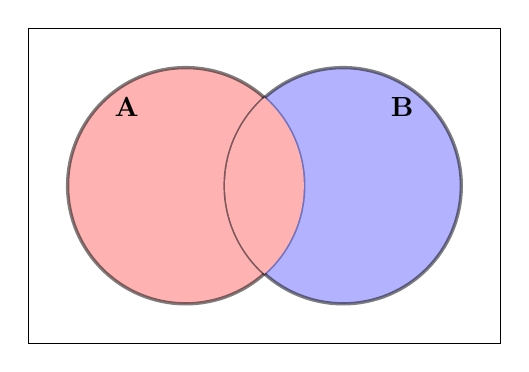
\begin{tikzpicture}
\def\circleA{(2,2) circle [radius = 1.5cm]} 
\def\circleB{(4,2) circle [radius = 1.5cm]} 
\draw (0,0) rectangle (6,4);

\onslide<3->{\draw[very thick, fill=red!60, opacity = 0.5] \circleA;
\node at (1.25,3) {\textbf{A}}; }

\onslide<4->{\draw[very thick, fill=blue!60, opacity = 0.5] \circleB;
\node at (4.75,3) {\textbf{B}}; }

\onslide<5->{
\begin{scope}[very thick]
\clip \circleA;
\fill[red!30] \circleB;
\end{scope} }

\end{tikzpicture} }
\end{center}
\end{frame}

\section{Calculate the complement of an event}

\section{Calculate "at least" probabilities}

\section{Calculate the odds of an event}

% Addition Rule
% General Addition Rule
% Complement Rule
% At least n
% Odds

\end{document}